\documentclass[a4paper]{article}
%\usepackage[singlespacing]{setspace}
\usepackage[onehalfspacing]{setspace}
%\usepackage[doublespacing]{setspace}
\usepackage{geometry} % Required for adjusting page dimensions and margins
\usepackage{amsmath,amsfonts,stmaryrd,amssymb,mathtools,dsfont} % Math packages
\usepackage{tabularx}
\usepackage{colortbl}
\usepackage{listings}
\usepackage{amsmath}
\usepackage{amssymb}
\usepackage{enumerate}
\usepackage{enumitem}
\usepackage{amsthm}
\usepackage{subcaption}
\usepackage{float}
\usepackage[table,xcdraw]{xcolor}
\usepackage{tikz-qtree}
\usepackage{forest}
\usepackage{changepage,titlesec,fancyhdr} % For styling Header and Titles
\pagestyle{fancy}
\renewcommand{\headrulewidth}{0.5pt} % Linienbreite anpassen, falls gewünscht
\renewcommand{\headrule}{
    \makebox[\textwidth]{\rule{1.0\textwidth}{0.5pt}} 
}
\usepackage{amsmath}
\pagestyle{fancy}
\usepackage{diagbox}
\usepackage{xfrac}

\usepackage{pgfplots}
\usepackage{pgfplotstable}
\pgfplotsset{compat=1.18}

\usepackage{enumerate} % Custom item numbers for enumerations

\usepackage[ruled]{algorithm2e} % Algorithms

\usepackage[framemethod=tikz]{mdframed} % Allows defining custom boxed/framed environments

\usepackage{listings} % File listings, with syntax highlighting
\lstset{
	basicstyle=\ttfamily, % Typeset listings in monospace font
}

\usepackage[ddmmyyyy]{datetime}


\geometry{
	paper=a4paper, % Paper size, change to letterpaper for US letter size
	top=3cm, % Top margin
	bottom=3cm, % Bottom margin
	left=2.5cm, % Left margin
	right=2.5cm, % Right margin
	headheight=25pt, % Header height
	footskip=1.5cm, % Space from the bottom margin to the baseline of the footer
	headsep=1cm, % Space from the top margin to the baseline of the header
	%showframe, % Uncomment to show how the type block is set on the page
}
\lhead{\vspace{0.5\baselineskip}Übungsblatt 2}
\chead{\bfseries{Einführung in Verteilte Systeme\\Sommersemester 2025}}
\rhead{\vspace{0.5\baselineskip}Werner, 7987847}
\fancyheadoffset[R]{0cm}

\begin{document}
\setcounter{section}{2}
\subsection{}
Gehen Sie von einer näherungsweisen Darstellung eines Rechtecksignals als Fourier-Reihe aus:
\[f(t)= \frac{4}{\pi}\sum\limits^\infty_{k=1}\frac{sin((2k-1)t)}{2k-1}=\frac{4}{\pi}\sum\limits^\infty_{k=1}a_k sin((2k-1)t)\]
\begin{enumerate}[label=\alph*)]
    \item Zeichnen Sie die Überlagerung entsprechend der Summe der Terme (für $k = 1, \dots , 4$)\\\\
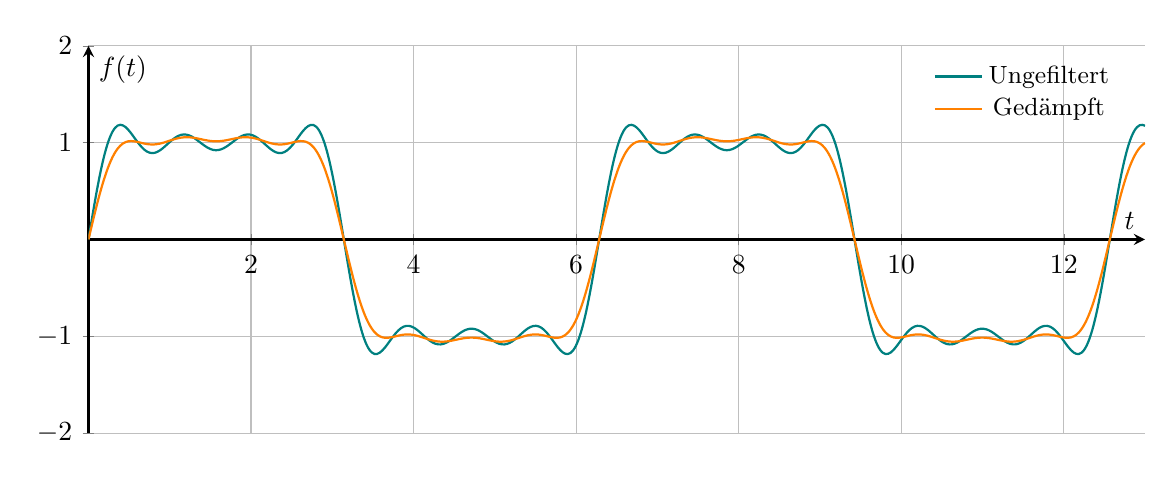
\begin{tikzpicture}
\begin{axis}[
    width=15cm,
    height=6.5cm,
    xlabel={$t$},
    ylabel={$f(t)$},
    grid=major,
    legend style={
        at={(0.98,0.98)},
        anchor=north east,
        draw=none,
        fill=none,
        font=\small
    },
    domain=0:13,
    samples=400,
    thick,
    axis lines=middle,
    ymin=-2, ymax=2,
    xtick={0,2,...,12},
    ytick={-2,-1,0,1,2},
    clip=true
]

% Ungedämpftes Signal (New color: Teal)
\addplot[
    teal,
    smooth
]
{(4/pi)*((sin(deg(x)) + sin(deg(3*x))/3 + sin(deg(5*x))/5 + sin(deg(7*x))/7))};
\addlegendentry{Ungefiltert}

% Gedämpftes Signal (New color: Orange)
\addplot[
    orange,
    smooth
]
{(4/pi)*((sin(deg(x)) + 0.8*sin(deg(3*x))/3 + 0.6*sin(deg(5*x))/5 + 0.4*sin(deg(7*x))/7))};
\addlegendentry{Gedämpft}

\end{axis}
\end{tikzpicture}

    \item Welche Frequenzen treten bei diesem Rechtecksignal auf, wenn man wieder die Terme für $k = 1, \dots , 4$ berücksichtigt?\\\\
    Der Term (2k - 1) bestimmt die Frequenzen. Diese sind:
    \begin{itemize}
        \item $\frac{1}{2\pi}$
        \item $\frac{3}{2\pi}$
        \item $\frac{5}{2\pi}$
        \item $\frac{7}{2\pi}$
    \end{itemize}
    \item Warum wird man ein perfektes Rechtecksignal in der Praxis nie erzeugen können?\\\\
    Ist unmóglich weil in der Parxis müssten die Flaken unendlich schnell und die Frequenzen unendlich hoch sein. Außerdem müssen die Frequenzen unendlich genau und konsistent sein. Demnach nicht möglich.
    \item Bei der Übertragung eines Funksignals über einen Kanal werden verschiedene Frequenzen unterschiedlich stark gedämpft. Gehen Sie von einer stärkeren Dämpfung bei höheren Frequenzen aus, entsprechend $a'_2 = 0.8 a_2,\, a'_3 = 0.6 a_3$ und $a'_4 = 0.4 a_4$, mit obigen Fourierkoeffizienten $a_k$. Wie wirkt sich dies auf die Form des Signals aus?\\\\
    Durch das Glätten wird die Kurve geglättet, also Steigungsunterschiede werden weniger rasant. Die Kurve ähnelt dadurch mehr einer Sinuskurve.
\end{enumerate}
\subsection{}
In der folgenden Graphik ist ein kontinuierliches Zeitsignal mit Periodendauer $T = 1/f$ gegeben.\\\\
Beim Sampling im Zuge der Digitalisierung dieses Signals sollen verschiedene Abtastfrequenzen $f_S$ untersucht und deren Ergebnisse gezeichnet werden. Die Signalabtastung soll jeweils beim
Zeitnullpunkt beginnen.\\\\
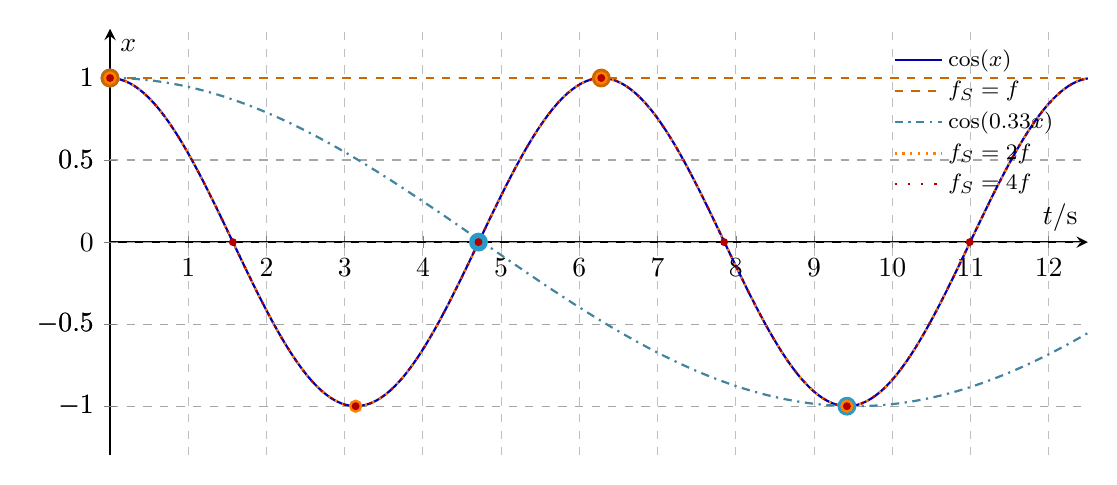
\begin{tikzpicture}
\begin{axis}[
    width=14cm,
    height=7cm,
    xlabel={$t/\mathrm{s}$},
    ylabel={$x$},
    domain=0:12.5,
    samples=200,
    axis lines=middle,
    ymin=-1.3, ymax=1.3,
    xmin=0, xmax=12.5,
    grid=major,
    grid style={dashed, gray!50},
    ytick={-1, -0.5, 0, 0.5, 1},
    extra y ticks={-1, -0.5, 0, 0.5, 1},
    extra y tick style={grid style={dashed, gray!70}},
    thick,
    legend style={
        at={(0.98,0.98)},
        anchor=north east,
        draw=none,
        fill=none,
        font=\footnotesize,
        legend cell align=left
    }
]

% Cosine wave (original)
\addplot[blue!70!black, thick] {cos(deg(x))};
\addlegendentry{$\cos(x)$}

% Constant line
\addplot[orange!80!black, dashed] {1};
\addlegendentry{$f_S = f$}

% Slower cosine
\addplot[cyan!60!black, dashdotted, thick] {cos(deg(0.33*x))};
\addlegendentry{$\cos(0.33x)$}

% Cosine sampled at 2f
\addplot[orange, dotted, thick] {cos(deg(x))};
\addlegendentry{$f_S = 2f$}

% Cosine sampled at 4f
\addplot[red!70!black, loosely dotted] {cos(deg(x))};
\addlegendentry{$f_S = 4f$}

% Sampled points (3 different sets)
\addplot[
    only marks,
    mark=*,
    mark size=3pt,
    cyan!80!black
]
table {
0   1
4.71   0
9.42   -1
};

\addplot[
    only marks,
    mark=*,
    mark size=3pt, 
    orange!80!black,
]
table {
0.0   1
6.28    1
12.56   1
};

\addplot[
    only marks,
    mark=*,
    mark size=2pt, 
    orange,
]
table {
0.0   1
3.14    -1
6.28    1
9.42    -1
12.56   1
};

\addplot[
    only marks,
    mark=*,
    mark size=1pt, 
    red!70!black,
]
table {
0.0     1
1.57    0
3.14    -1
4.71    0
6.28    1
7.85    0
9.42    -1
10.99   0
12.56   1
};

\end{axis}
\end{tikzpicture}

\begin{enumerate}[label=\alph*)]
    \item Überführen Sie das Orignalsignal jeweils in eine diskrete Form bei einer Abtastrate von
    \begin{itemize}
        \item $f_S=f=1$
        \item $f_S=\frac{4}{3}f=cos(\frac{x}{}x)$
        \item $f_S=2f=cos(x)$
        \item $f_S=4f=cos(x)$
    \end{itemize}
    Geben Sie die Ergebnisse numerisch und graphisch an.\\\\
    Die Funktionen sind im Graphen überführt.\\
    \item Formulieren Sie das Theorem von Shannon für die Abtastung eines Signals in ein bis zwei Sätzen.\\\\
    Ein kontinuierliches Signal mit maximaler Frequenz $f_{max}$ kann verlustfrei rekonstruiert werden, wenn die Abtastfrequenz $f_s$ mindestens das Doppelte von $f_{max}$ beträgt.
\end{enumerate}
\end{document}
